%% ISU-Challenge @ ICSE 2027, Track B -- participant tool report (27 Nov 2026).
%% IEEE conference format (IEEEtran), four pages including references.
%% Every number comes from numbers.tex / tab_*.tex / figures/*, generated by
%% compute_metrics.py, make_tables.py and make_figures.py from the saved run artefacts.
\documentclass[10pt,conference]{IEEEtran}

\usepackage[T1]{fontenc}
\usepackage{cite}
\usepackage{amsmath}
\usepackage{graphicx}
\usepackage{booktabs}
\usepackage{url}
\newcommand{\nAll}{10{,}749}
\newcommand{\nReal}{479}
\newcommand{\nSyn}{10{,}270}
\newcommand{\vTwoCorrect}{10{,}748}
\newcommand{\vOneCorrect}{10{,}747}
\newcommand{\vTwoLat}{41}
\newcommand{\vOneLat}{32}
\newcommand{\ensLat}{67}
\newcommand{\nParams}{89.0}
\newcommand{\nParamsBB}{86.6}
\newcommand{\nParamsHead}{2.44}
\newcommand{\sOneEpochs}{6}
\newcommand{\sTwoSteps}{400}
\newcommand{\batch}{32}
\newcommand{\sOneBbLr}{5\times10^{-5}}
\newcommand{\layerDecay}{0.8}
\newcommand{\weightDecay}{0.05}
\newcommand{\emaOne}{0.998}
\newcommand{\emaTwo}{0.99}
\newcommand{\nHoldout}{500}
\newcommand{\nHoldoutAns}{10{,}392}
\newcommand{\nCvAns}{478}
\newcommand{\vTwoTrainH}{3.9}
\newcommand{\vTwoMinMargin}{5.3}
\newcommand{\graphEager}{69.7}
\newcommand{\graphGraph}{71.4}

\emergencystretch=1.5em % lets lines with long hyphenated terms break inside the column
\newcommand{\tool}{CabinQ}% name of the tool; change here only

\begin{document}

\title{\tool{} at the ISU-Challenge 2027: Fast In-Car Scene Understanding with One Learned Query per Question}

\author{\IEEEauthorblockN{Dandu Venkata Nitish Chandra Teja}
\IEEEauthorblockA{Amrita Vishwa Vidyapeetham\\
Coimbatore, India\\
dandunitish@gmail.com}}

\maketitle

\begin{abstract}
This report presents \tool{}, a tool for in-car scene understanding developed for Track B of the ISU-Challenge at ICSE 2027. Given a single RGB image of a car cabin, \tool{} answers 31 questions about occupants, seat belts, phone use, and objects in one forward pass, using a DINOv2-B/14 backbone with one learned query per question. It is trained first on synthetic renders and then, once per cross-validation fold, on renders mixed with the 30 public real photos; the fold models are averaged into a single model. In the official evaluation, \tool{} answers \vTwoCorrect{} of \nAll{} questions correctly, with one error on real photos, at \vTwoLat{}~ms per image on an NVIDIA L4 GPU. We describe the tool, its evaluation, and the evolution of the solution, and show that with only 30 real photos the random seed alone changes the cross-validated error count from 1 to 6.
\end{abstract}

\begin{IEEEkeywords}
in-car scene understanding, vision transformers, sim-to-real transfer, multi-label classification, weight averaging
\end{IEEEkeywords}

\section{Introduction}
In-cabin monitoring systems use camera images to detect safety-relevant situations, such as unbelted occupants or a driver using a phone. Track B of the ISU-Challenge targets such systems: given a single RGB image of a car interior, a system has to answer a fixed set of questions about the scene~\cite{sorokin2026isutest}. Each of the 31 scored questions has exactly two admissible answers. The available training data comprise about 6{,}000 labeled synthetic renders and 30 labeled real photos.

The baseline of the starter kit relies on a general-purpose vision-language model~\cite{bai2025qwen25vl}. In contrast, \tool{} treats the task as multi-label binary classification: since both the questions and the admissible answers are fixed, a specialized classifier can answer all questions in a single forward pass, with a score for every answer and a latency of a few tens of milliseconds. The main challenge is not the synthetic domain, which a strong pretrained backbone learns almost perfectly, but the transfer to real photos, of which only 30 are available for training.

This report presents the tool (Section~\ref{sec:tool}), the experimental setup used during development (Section~\ref{sec:setup}), and the results, including the evolution of the solution and the variants that did not improve it (Section~\ref{sec:results}). Section~\ref{sec:conclusions} concludes the report.

\begin{figure}[t]
  \centering
  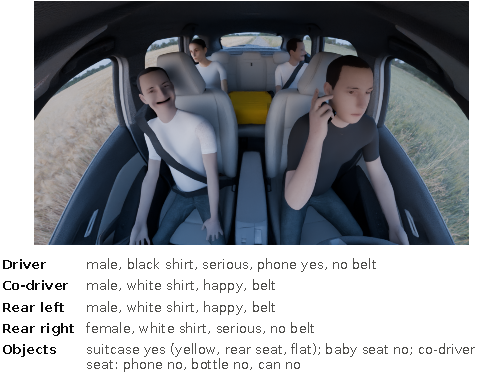
\includegraphics[width=\columnwidth]{figures/fig_teaser.pdf}
  \caption{A synthetic render from our hold-out set, which \tool{} did not see during training, and the answers produced by \tool{} (28 of 28 labeled questions correct).}
  \label{fig:teaser}
\end{figure}

\section{The \tool{} Tool}\label{sec:tool}
\subsection{Task Formulation}
We map the two admissible answers of each question to 0 and 1. \tool{} therefore produces 31 sigmoid outputs, and every prediction is a valid answer by construction. Some labels are undefined, e.g., the shirt color of an absent co-driver; such entries are masked out of the loss. At inference time, \tool{} answers all 31 questions and ignores the text prompt passed by the evaluation pipeline, as the question set is fixed.

\subsection{Model Architecture}
Figure~\ref{fig:method} gives an overview of the architecture.

\textbf{Backbone.} \tool{} uses DINOv2-B/14~\cite{oquab2024dinov2}, a Vision Transformer~\cite{dosovitskiy2021vit} pretrained with self-supervision. Images are resized to 952$\times$532 pixels, the native resolution of the renders, which yields 68$\times$38 patch tokens of 14$\times$14 pixels plus a CLS token.

\textbf{Query head.} The head holds one learned query vector per question. A single multi-head cross-attention layer with eight heads lets each query attend to all image tokens; it is followed by a residual connection, layer normalization, and a linear read-out per question. A linear projection of the CLS token is added to all outputs. Learned queries with cross-attention follow DETR~\cite{carion2020detr} and Query2Label~\cite{liu2021query2label}. The rationale is locality: the query for, e.g., the rear-right seat belt can focus on that seat, whereas a pooled image feature mixes all seats. The model has \nParams{}\,M parameters, \nParamsHead{}\,M of which belong to the head.

\begin{figure}[t]
  \centering
  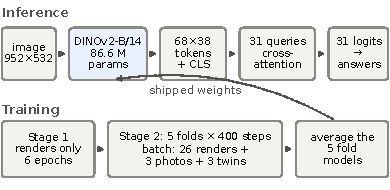
\includegraphics[width=\columnwidth]{figures/fig_method.pdf}
  \caption{Overview of \tool{}. Top: a single forward pass answers all questions. Bottom: the two training stages and the weight averaging that produces the submitted model.}
  \label{fig:method}
\end{figure}

\subsection{Training Procedure}
\textbf{Stage 1} trains on synthetic renders only. We hold out \nHoldout{} renders (\nHoldoutAns{} labeled answers) for testing and train on the remaining 5{,}500 renders for \sOneEpochs{} epochs with a batch size of \batch{}. We use AdamW~\cite{loshchilov2019adamw} with a weight decay of \weightDecay{}, layer-wise learning-rate decay of \layerDecay{}~\cite{bao2022beit}, a cosine schedule, and a backbone learning rate of $\sOneBbLr$. The backbone is frozen during the first 150 steps so that the randomly initialized head does not disturb the pretrained features, and an exponential moving average (EMA) of the weights with a decay of \emaOne{} is used for evaluation~\cite{tarvainen2017meanteacher}. Data augmentation imitates camera variation: small changes in scale, rotation, and position, as well as in white balance, exposure, contrast, gamma, blur, sensor noise, and resolution. Horizontal flips are excluded, as they would swap the driver and co-driver labels, and so are hue changes, as colors are labels.

\textbf{Stage 2} adapts the model to real photos. The 30 real photos are split into five folds, stratified on the four questions that are hardest on real photos (driver phone, driver belt, driver emotion, and baby seat). For each fold, training restarts from the stage-1 weights and runs for \sTwoSteps{} steps with lower learning rates ($1.5\times10^{-5}$ for the backbone, $1.5\times10^{-4}$ for the head) and an EMA decay of \emaTwo{}. Each batch contains 26 renders, 3 real photos from the four training folds, and 3 \emph{twins}, i.e., renders of the scenes depicted in the photos of those folds. In this way, the model sees the same scenes in both their rendered and their real appearance, while the renders keep the synthetic domain represented.

\textbf{Weight averaging.} The submitted model is the uniform average of the five fold models, i.e., a model soup~\cite{wortsman2022soups}. As all fold models start from the same stage-1 weights, their average remains a well-performing model. In addition, each fold model is evaluated on the photos it did not train on (Section~\ref{sec:setup}). Training uses mixed precision~\cite{micikevicius2018mixed} and gradient checkpointing~\cite{chen2016checkpoint} and takes \vTwoTrainH{}~h on two NVIDIA T4 GPUs.\footnote{Training was run on Kaggle with two NVIDIA T4 GPUs, PyTorch 2.11, and Transformers 4.57.6~\cite{wolf2020transformers}; the official evaluation runs on an NVIDIA L4 GPU.}

\subsection{Inference}
Training and inference share the same preprocessing module, so the submitted system receives exactly the pixel values seen during training. Inference runs in half precision on the GPU, without test-time augmentation. A wrapper safeguards the evaluation run: if the model cannot be loaded, the system fails at start-up, so that the problem surfaces in the free preflight check rather than in a scored evaluation; if a GPU call fails, the model is reloaded on the CPU; and if this fails as well, the system returns the most frequent answer for each question. All returned values are checked against the admissible answers.

\begin{figure*}[t]
  \centering
  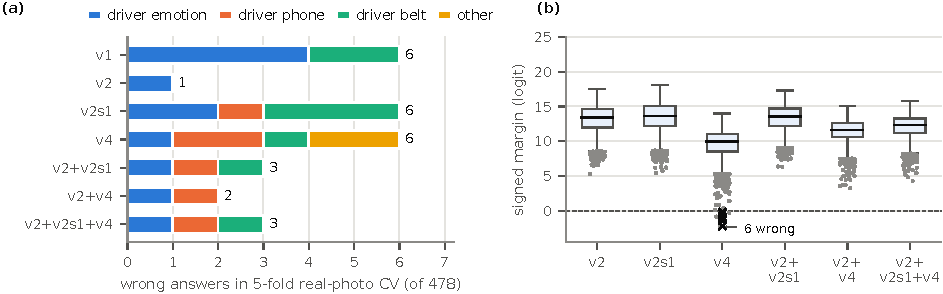
\includegraphics[width=\textwidth]{figures/fig_results.pdf}
  \caption{Development results. (a) Wrong answers in the real-photo cross-validation, by question. (b) Signed margins on the synthetic hold-out (box: quartiles; whiskers: 1st--99th percentile; dots: the lowest 1\%; crosses: wrong answers).}
  \label{fig:results}
\end{figure*}

\section{Experimental Setup}\label{sec:setup}
\subsection{Evaluated Variants}
We refer to our training runs by version numbers. Unless stated otherwise, all variants share the architecture and training procedure of Section~\ref{sec:tool}.
\textbf{v1}, our first submission, uses an input size of 644$\times$364 and 12 stage-1 epochs.
\textbf{v2}, our final submission, is the configuration described in Section~\ref{sec:tool} (952$\times$532 pixels, \sOneEpochs{} stage-1 epochs).
\textbf{v2s1} is identical to v2 except for the random seed, which changes the weight initialization, data order, augmentation, and stage-2 sampling, while the data splits remain the same.
\textbf{v4} follows the v2 procedure with a DINOv3-B/16 backbone~\cite{simeoni2025dinov3} at 1088$\times$608 pixels, which yields the same 68$\times$38 token grid as v2, and 3 stage-1 epochs.
\textbf{Ensembles}, written as v2\,+\,v4, average the logits of their members. A planned v3 with a DINOv2-L backbone was not trained.

\subsection{Metrics}
\emph{Accuracy.} The official evaluation reports the number of correct answers, separately for real photos and renders, as well as the number of scenes answered without error.
\emph{Errors and log-loss.} During development, we count wrong answers and compute the log-loss of the predicted probabilities.
\emph{Signed margin.} The signed margin of an answer is its logit multiplied by $+1$ if the answer is correct and by $-1$ otherwise; values close to zero indicate answers that could flip under small changes of the input.
\emph{Latency.} The mean time per image measured by the official evaluation.

\subsection{Procedure}
We evaluated each variant on two internal test sets, one per domain. The \emph{synthetic hold-out} consists of the \nHoldout{} renders excluded from training. For the \emph{real-photo cross-validation} (CV), each of the 30 photos is answered by the fold model that did not train on it, which yields \nCvAns{} labeled answers. Variants without any synthetic hold-out error were submitted to the official evaluation, which allows three runs per day.

\begin{table}[t]
\caption{Official evaluation results of the submitted variants on an NVIDIA L4: correct answers out of 10{,}749 (479 on real photos, 10{,}270 on renders), real scenes answered without error, and mean latency per image. Bold indicates the best values.}
\label{tab:official}
\small
\begin{tabular}{@{}lcrrrcr@{}}
\toprule
System & PR & All & Real & Synth. & Real exact & s/img \\
\midrule
v1 & \#34 & 10{,}747 & 477 & \textbf{10{,}270} & 28/30 & \textbf{0.032} \\
v2 (final) & \#35 & \textbf{10{,}748} & \textbf{478} & \textbf{10{,}270} & \textbf{29/30} & 0.041 \\
v2 + v2s1 & \#38 & \textbf{10{,}748} & \textbf{478} & \textbf{10{,}270} & \textbf{29/30} & 0.067 \\
v2 + v4 & \#39 & \textbf{10{,}748} & \textbf{478} & \textbf{10{,}270} & \textbf{29/30} & 0.067 \\
\bottomrule
\end{tabular}
\end{table}


\section{Results}\label{sec:results}
\subsection{Official Evaluation}
Table~\ref{tab:official} reports the official evaluation results. Our final variant, v2, answers \vTwoCorrect{} of \nAll{} questions correctly: all \nSyn{} answers on renders and 478 of \nReal{} answers on real photos, such that 29 of the 30 real scenes are answered without error. Its mean latency is \vTwoLat{}~ms per image on the L4.

\begin{table}[t]
\caption{Development results. Synthetic hold-out: errors and smallest signed margin (logits) over 10{,}392 answers on 500 unseen renders. Real-photo CV: errors and log-loss over 478 answers. Training time in hours on 2$\times$T4; margin and log-loss are unavailable for v1. Bold indicates the best values.}
\label{tab:dev}
\footnotesize
\setlength{\tabcolsep}{4pt}
\begin{tabular}{@{}lcrrrrr@{}}
\toprule
& & \multicolumn{2}{c}{Synth.\ hold-out} & \multicolumn{2}{c}{Real-photo CV} & Train \\
\cmidrule(lr){3-4}\cmidrule(lr){5-6}
Variant & Input & errors & margin & errors & log-loss & h \\
\midrule
v1 & 644$\times$364 & \textbf{0} & -- & 6 & -- & 1.6 \\
v2 & 952$\times$532 & \textbf{0} & $5.3$ & \textbf{1} & 0.011 & 3.9 \\
v2s1 & 952$\times$532 & \textbf{0} & $5.5$ & 6 & 0.043 & 3.5 \\
v4 & 1088$\times$608 & 6 & $-2.2$ & 6 & 0.028 & 3.5 \\
\midrule
v2 + v2s1 & -- & \textbf{0} & \textbf{6.3} & 3 & 0.019 & -- \\
v2 + v4 & -- & \textbf{0} & 3.3 & 2 & \textbf{0.009} & -- \\
v2 + v2s1 + v4 & -- & \textbf{0} & 4.3 & 3 & 0.014 & -- \\
\bottomrule
\end{tabular}
\end{table}


\subsection{Development Results}
Table~\ref{tab:dev} reports the development results. v2 makes no error on the synthetic hold-out, and its smallest margin is \vTwoMinMargin{} logits, which corresponds to a probability above 0.99 for the correct answer. In the real-photo CV, it makes a single error out of \nCvAns{}: the driver's emotion on photo 4, in which the driver holds a phone and our face detector finds no face (Section~\ref{sec:evolution}). As shown in Figure~\ref{fig:results}a, all CV errors of all variants concern the driver's emotion, phone use, or seat belt, except for two answers of v4; these are the questions for which renders and real photos differ the most.

\subsection{Evolution of the Solution}\label{sec:evolution}
\emph{From v1 to v2.} v1 scored \vOneCorrect{} of \nAll{} at \vOneLat{}~ms, with six CV errors (four on the driver's emotion and two on the driver's belt). For v2, we raised the input size to the native render resolution, which provides the head with 2.2 times more tokens and finer detail for small cues, such as a dark belt on a dark shirt. We also shortened stage 1 to six epochs, as v1 had made only two hold-out errors after four epochs. The logs of v2 support this choice: before stage 2, its real-photo errors increased from 22 after three epochs to 27 after six, while its synthetic hold-out was already free of errors after three. v2 gained one correct answer in the official evaluation and reduced the CV errors from six to one. Since both settings changed at once and both gains are within the seed-to-seed variation discussed below, we cannot attribute the improvement to either change.

\emph{Variants that did not improve the results.} We explored four further directions. (i)~\emph{DINOv3 backbone}: after three stage-1 epochs, v4 made 21 hold-out errors, compared with none for v2 at the same point; after stage 2, the averaged model still made six errors, all on the rear-right passenger's emotion (Figure~\ref{fig:results}b), as well as six CV errors. (ii)~\emph{Ensembles}: averaging v2 with v2s1 or v4 removes all synthetic errors (Figure~\ref{fig:results}b), but both ensembles scored exactly like v2 in the official evaluation, at \ensLat{}~ms instead of \vTwoLat{}~ms, and made two to three CV errors instead of one. (iii)~\emph{Facial-expression expert}: we combined a face detector~\cite{wu2023yunet} with a facial-expression model~\cite{savchenko2022classifying} for the driver's emotion. The detector found a face in only 19 of the 30 real photos, as the camera looks down on the occupants, and fusing the expert's scores with v2 did not correct any of v2's CV errors. (iv)~\emph{Driver crop}: the driver's face is already about 126 pixels tall in v2's input (about 255 pixels in the original photo), so a separate high-resolution crop of the driver would add little detail; we therefore did not build it. Finally, capturing the forward pass as a CUDA graph produced identical outputs but no speed-up on the T4 (\graphGraph{} vs.\ \graphEager{}~ms), so the submitted system runs in eager mode.

\emph{Seed variation.} v2s1 differs from v2 only in its random seed. Its synthetic results are equally clean, but it makes six CV errors instead of one (Figure~\ref{fig:results}a). Hence, a single run per configuration cannot separate configurations that differ by a few real-photo errors, and the CV result of v2 is partly due to chance. The official results are consistent with this observation, as three different variants obtained \vTwoCorrect{} correct answers. Among them, we selected the fastest one, v2.

\section{Conclusions and Final Remarks}\label{sec:conclusions}
This report presented \tool{}, our tool for Track B of the ISU-Challenge. \tool{} shows that a fixed set of questions can be answered by a compact classifier: a self-supervised Vision Transformer, one learned query per question, two-stage training, and five-fold weight averaging achieve \vTwoCorrect{} of \nAll{} correct answers at \vTwoLat{}~ms per image. The synthetic domain is solved; the remaining errors occur on real photos and concern the driver's emotion, phone use, and seat belt. With only 30 real photos, a reliable comparison of variants requires several seeds per configuration or additional real data.

\emph{Limitations.} Our real-photo estimates rest on 30 photos, all taken in a garage with only the driver on board, so the CV does not test passengers or objects on real photos. The withheld real photos depict scenes whose published renders were part of our training data (24 of these 30 renders were used in stage 1; the withheld photos themselves were never used). The official real-photo score may therefore be more favorable than the CV, in which no fold model trains on the render of a photo it is tested on. Moreover, the official evaluation reports totals only, so we do not know which real-photo answer v2 gets wrong, and latency was measured on the L4 used for the leaderboard; other GPUs yield different times.

\emph{Reproducibility.} All runs use fixed random seeds and the same data splits, pin the versions of the model libraries (Transformers, timm), and share the preprocessing code with the submitted system. Before each submission, we verified on a local CPU that the downloaded weights reproduce the errors reported during training on the real photos, and we logged SHA-256 hashes of all submitted files. Retraining v2 takes about \vTwoTrainH{}~h on two T4 GPUs.

%% Replication package; the trained weights are attached to its release "weights-v1".
\emph{Availability.} The training and inference code, run logs, trained weights, and the scripts that generate all numbers in this report are available at \url{https://github.com/invst-git/cabinq-isu-track-b}.

\section*{Acknowledgment}
We thank the organizers of the ISU-Challenge for providing the dataset, the starter kit, and the evaluation infrastructure, and Kaggle for the GPU time used for training.

\bibliographystyle{IEEEtran}
\bibliography{refs}

\end{document}
